\documentclass[11pt]{article}
\usepackage[margin=1in]{geometry}
\usepackage{amsmath,amssymb,mathtools}
\usepackage{booktabs}
\usepackage{microtype}
\usepackage{hyperref}
\usepackage{tikz}
\usepackage{pgfplots}
\usepgfplotslibrary{fillbetween}
\pgfplotsset{compat=1.18}
\hypersetup{colorlinks=true,linkcolor=blue!50!black,citecolor=blue!50!black,urlcolor=blue!50!black}

\newcommand{\kb}{k_{\mathrm B}}
\newcommand{\Tpair}{T_{\mathrm{pair}}}
\newcommand{\Tlin}{T_{\mathrm{lin}}}
\newcommand{\taui}{\tau_*}
\newcommand{\DOI}[1]{\href{https://doi.org/#1}{#1}}
\newcommand*{\CAPSTONEDOI}{10.5281/zenodo.24406996}
\newcommand*{\CAPSTONEREPO}{https://github.com/SuperMatics-Inc/phonon-pairing-ceiling-map}

\title{Rigorous ceilings on phonon-mediated pairing:\\ a map from Eliashberg theory to the Holstein model}
\author{Davis Rens\\SuperMatics Inc.\\\href{https://orcid.org/0000-0001-5839-5197}{ORCID 0000-0001-5839-5197}}
\date{\parbox{.98\linewidth}{\centering\scriptsize
20 November 2026\qquad Article DOI: \href{https://doi.org/10.5281/zenodo.24406996}{\CAPSTONEDOI}\\
Source repository: \expandafter\url\expandafter{\CAPSTONEREPO}
}}

\begin{document}
\maketitle

\begin{abstract}
A familiar phenomenological shorthand places a conventional phonon pairing temperature at a scale of roughly one tenth of a characteristic phonon energy. A theorem matching that scale for an exact lattice Hamiltonian at all couplings is not presently available. This paper organizes released upper bounds into two distinct layers. In linearized Eliashberg theory, successive moment estimates reduce the coefficient multiplying the square root of the glue moment. For the square-lattice Holstein model, exponential clustering gives an implicit two-thirds-power frequency bound, while a separate strong-coupling theorem gives a frequency-uniform ceiling proportional to $t^2/U$. Their minimum yields a regime map and leaves a low-frequency strip in which the two-thirds-power estimate is the stronger result. Determinant-zero witnesses obstruct a specified family of per-history arguments, not every route to a linear ceiling. The final section states the remaining linear-in-frequency conjecture without asserting it.
\end{abstract}

\section{Introduction}

The compact rule of thumb $\kb T_c\lesssim0.1\bar\Omega$, with $\bar\Omega$ a characteristic phonon energy, is useful as phenomenological orientation. Its numerical meaning depends on the choice of frequency average, the Coulomb contribution, and the regime of the coupling. Strong-coupling formulas clarify this dependence but do not themselves furnish an exact-Hamiltonian theorem for local pair correlations; see, for example, the Eliashberg-based analyses of McMillan and Allen and Dynes~\cite{mcmillan,allendynes}. We use the shorthand as motivation, not as a universal inequality.

There are two mathematical questions to keep separate. Linearized Eliashberg theory studies instability of a specified normal branch to an infinitesimal pairing perturbation. The lattice results below instead control correlations of electronic operators in the full electron-phonon Gibbs state. A ceiling on the former is not, without a model-specific argument, a ceiling on the latter. The purpose here is to put the released results side by side and make their domains of control visible.

Write $\tau=\kb T$. In the Holstein model, $t>0$ is the bare nearest-neighbour hopping, $U=F^2/K>0$ is the oscillator relaxation energy, and $\Omega=\hbar\sqrt{K/m}>0$ is the phonon energy. The pair temperature $T_{\mathrm{pair}}$ refers to the supremum of temperatures at which a fixed finite-support electronic charge-two field can have algebraic equal-time correlations in the thermodynamic limit, using the convention in the clustering theorem. It is not identified with an Eliashberg onset temperature. Unless specified otherwise, statements for Holstein are for the spinful square-lattice model without a direct electron interaction.

\section{The Eliashberg layer}

The relevant control parameter is a norm $\rho$ of the retarded glue moment, not a phonon-only average. The released centered-branch theorem gives
\[
 \kb\Tlin < C_{\mathrm U}\sqrt{\rho},\qquad
 C_{\mathrm U}=\frac{1}{2\pi}\sqrt{\frac{6466219}{3576050}}\simeq0.2140146706,
\]
under its finite-channel hypotheses: nonnegative integrable even channel densities bounded by their channel heights, no real normal shifts, and a reciprocal positive Lorentzian-mixture normal kernel with bounded folded rows dominating the pairing envelope~\cite{univglue}. This is a valid upper bound for that class, not a claim that its coefficient is sharp.

Under the stated model and branch hypotheses of the multipoint multichannel ceiling~\cite{optimum}, retaining twenty tail frequencies improves the coefficient to
\[
 \kb\Tlin < C_{21}\sqrt{\rho},\qquad
 C_{21}=\frac{\sqrt{377/250}}{2\pi}\simeq0.19544330695.
\]
For channel- and energy-dependent densities of states, the two-stage refinement~\cite{finiteenergy} yields
\[
 \kb\Tlin < C\sqrt{\rho},\qquad
 C=\begin{cases}
 \displaystyle\frac{\sqrt{41/30}}{2\pi}\simeq0.1860593214,&\text{centered normal branch},\\[5pt]
 \displaystyle\frac{\sqrt{45/32}}{2\pi}\simeq0.1887345454,&\text{causal branch}.
 \end{cases}
\]
These inequalities concern linearized pairing stability on the stated branches. The constants form a rigorous progression within their respective hypotheses, rather than a conversion from $\rho$ to the $\Omega$ of a particular lattice Hamiltonian.

\begin{table}[ht]
\centering
\caption{Released Eliashberg ceilings. Each citation identifies the corresponding Zenodo record.}
\begin{tabular}{@{}lll@{}}
\toprule
Result & Coefficient of $\sqrt{\rho}$ & Zenodo record\\
\midrule
Universal glue, centered class & $\sqrt{6466219/3576050}/(2\pi)$ & \cite{univglue}\\
Multipoint multichannel bound & $\sqrt{377/250}/(2\pi)$ & \cite{optimum}\\
Energy-dependent DOS, centered class & $\sqrt{41/30}/(2\pi)$ & \cite{finiteenergy}\\
Energy-dependent DOS, causal class & $\sqrt{45/32}/(2\pi)$ & \cite{finiteenergy}\\
\bottomrule
\end{tabular}
\end{table}

\section{The model layer: Holstein and bond SSH}

For the spinful square-lattice Holstein and bond Su--Schrieffer--Heeger (SSH) models with independent harmonic phonons and no direct electron interaction, the released two-thirds clustering theorem gives exponential clustering above the threshold
\begin{equation}\label{eq:two-thirds}
 \tau^3\geq 2^{25}U\Omega^2\left[1+\log\left(1+\frac{E}{\tau}\right)\right],
 \qquad E=\begin{cases}t,&\text{Holstein},\\t+U,&\text{bond SSH}.
 \end{cases}
\end{equation}
Consequently $\kb\Tpair\leq\taui$, where $\taui$ is the unique positive solution of equality in~\eqref{eq:two-thirds}. At fixed $t,U>0$ and small $\Omega$, this threshold has scale $\Omega^{2/3}[\log(E/\Omega)]^{1/3}$, with a parameter-dependent prefactor. The theorem applies to specified fixed-support electronic fields and gives uniform clustering in the stated grand-canonical and thermodynamic canonical settings~\cite{linear4}.

A different theorem applies to the on-site Holstein pair field
\[
 \Delta_x=c_{x\downarrow}c_{x\uparrow},
\]
at strong coupling and is uniform in every positive phonon frequency. If
\[
 \frac{\beta t^2}{U}\leq 2^{-27},
\]
then for distinct $x,y$,
\[
 \bigl|\langle\Delta_x^\dagger\Delta_y\rangle\bigr|
 \leq \frac{240}{59}\left(\frac{5}{64}\right)^{d(x,y)}.
\]
In particular, for pair order defined by this field,
\begin{equation}\label{eq:strong-coupling}
 \kb\Tpair^{\mathrm{on\text{-}site}}\leq 2^{27}\frac{t^2}{U}.
\end{equation}
No restriction on the ratio $t/U$ is added beyond the displayed temperature condition. This is a Holstein result; it is not an SSH estimate~\cite{stage6}.

The two theorems answer complementary questions. The two-thirds threshold improves as $\Omega$ decreases, but only with exponent $2/3$ up to a logarithm. The uniform-frequency strong-coupling threshold does not depend on $\Omega$ and can be restrictive in a strong-coupling, low-temperature regime. Taking the smaller available bound gives a rigorous envelope without identifying either estimate with the actual transition temperature. The combined envelope in Section 4 and Fig.~\ref{fig:map} applies to the on-site field $\Delta_x=c_{x\downarrow}c_{x\uparrow}$; Eq.~\eqref{eq:two-thirds} alone covers general fixed-support charge-two fields.

\section{A theorem map in the \texorpdfstring{$(t/U,\Omega/t)$}{(t/U, Omega/t)} plane}

Set $x=t/U$, $y=\Omega/t$, and $z=\tau/t$. For the on-site pair field in the Holstein model, the two-thirds boundary is the positive solution $z_{2/3}(x,y)$ of
\begin{equation}\label{eq:z-two-thirds}
 z_{2/3}^3=2^{25}x^{-1}y^2\left[1+\log\left(1+\frac{1}{z_{2/3}}\right)\right],
\end{equation}
whereas the uniform-frequency strong-coupling theorem gives $z_{\mathrm{sc}}(x)=2^{27}x$. Equating these exact expressions gives the crossover curve
\begin{equation}\label{eq:crossover}
 y_c(x)=\frac{2^{28}x^2}{\sqrt{1+\log\left(1+(2^{27}x)^{-1}\right)}}.
\end{equation}
For $y\leq y_c(x)$ the two-thirds threshold is the smaller one; for $y\geq y_c(x)$ the uniform-frequency strong-coupling threshold is the smaller one. Figure~\ref{fig:map} displays that comparison on a finite logarithmic window. The colors encode which of these two ceilings is tighter, not physical phases or order parameters.

\begin{figure}[ht]
\centering
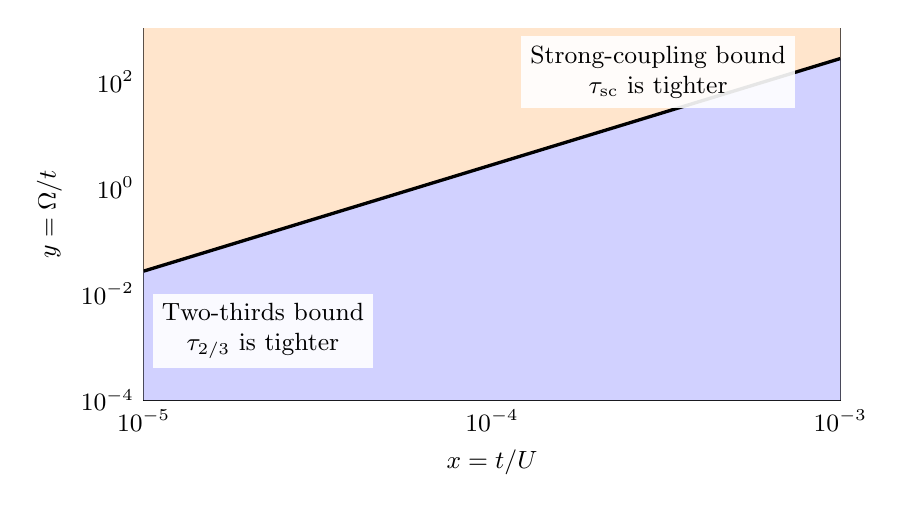
\begin{tikzpicture}
\begin{axis}[
 width=0.86\textwidth,
 height=0.52\textwidth,
 xmode=log, ymode=log,
 xmin=1e-5, xmax=1e-3,
 ymin=1e-4, ymax=1e3,
 xlabel={$x=t/U$}, ylabel={$y=\Omega/t$},
 xtick={1e-5,1e-4,1e-3},
 ytick={1e-4,1e-2,1,1e2},
 grid=major,
 tick label style={font=\small},
 label style={font=\small},
 clip=true
]
\addplot[draw=none,name path=boundary,domain=0:2,samples=201]
({10^(-5+x)}, {2^28*(10^(-5+x))^2/sqrt(1+ln(1+1/(2^27*(10^(-5+x))))) });
\addplot[draw=none,name path=bottom] coordinates {(1e-5,1e-4) (1e-3,1e-4)};
\addplot[draw=none,name path=top] coordinates {(1e-5,1e3) (1e-3,1e3)};
\addplot[blue!18] fill between[of=boundary and bottom];
\addplot[orange!20] fill between[of=boundary and top];
\addplot[black,very thick,domain=0:2,samples=201]
({10^(-5+x)}, {2^28*(10^(-5+x))^2/sqrt(1+ln(1+1/(2^27*(10^(-5+x))))) });
\node[fill=white,fill opacity=0.9,text opacity=1,align=center,font=\small] at (axis cs:2.2e-5,2e-3) {Two-thirds bound\\$\tau_{2/3}$ is tighter};
\node[fill=white,fill opacity=0.9,text opacity=1,align=center,font=\small] at (axis cs:3e-4,1.5e2) {Strong-coupling bound\\$\tau_{\mathrm{sc}}$ is tighter};
\end{axis}
\end{tikzpicture}
\caption{Comparison of the Holstein on-site pair bounds on $10^{-5}\leq t/U\leq10^{-3}$ and $10^{-4}\leq\Omega/t\leq10^3$. The black curve is the exact crossover~\eqref{eq:crossover}; below it $\tau_{2/3}\leq\tau_{\mathrm{sc}}$, and above it $\tau_{\mathrm{sc}}\leq\tau_{2/3}$. Here $\tau_{2/3}=t z_{2/3}$ is determined implicitly by~\eqref{eq:z-two-thirds} and $\tau_{\mathrm{sc}}=2^{27}t^2/U$. The figure is a theorem map, not a physical phase diagram.}
\label{fig:map}
\end{figure}

\section{The remaining low-frequency strip}

Fix $t,U>0$, so that $x$ is fixed. As $\Omega\downarrow0$, $y$ eventually lies below $y_c(x)$. In that strip the uniform-frequency strong-coupling estimate~\eqref{eq:strong-coupling} no longer supplies the smaller ceiling; the available square-lattice estimate is the two-thirds clustering scale in~\eqref{eq:two-thirds}. Its $\Omega^{2/3}$ behavior is stronger than the static square-root estimate~\cite{slowphonon}, but it is not linear in $\Omega$. The gap is a limitation of the proved bounds, not evidence for a physical transition at either threshold.

A separate analysis gives positive imaginary-time estimates and method-specific barriers beyond the two-thirds scale, without resolving the model-level linear target~\cite{linear5}. The two-thirds clustering proof conditions on a static oscillator background while retaining bounded time-dependent histories in the electronic reference. A companion determinant analysis exhibits a six-piece zero-mean history on a four-site $K_{1,3}$ star that drives the single-spin determinant through zero with dimensionless field norm below five at tested values of $\beta t$; the normalized one-spin Green function is singular there. For~\mbox{$\beta t\geq40$}, uniform invertibility within this family requires a sup-norm cutoff $\kappa<5$, while its free-law Peierls-weight estimate requires $\tau^3\gtrsim U\Omega^2/(12\kappa^2)$, retaining the two-thirds scale. This restriction applies to the specified cutoff family and does not exclude other per-history estimates or a linear model-level bound~\cite{barriers}.

A complementary gap-conditioned theorem assumes $t\leq g/64$ and $2^{10}\sqrt{U/g}\,\Omega\leq\tau\leq g$. Under conditioning that all static fields are $g$-gapped, it gives exponential clustering for fixed-support monomials of opposite nonzero even charge. The companion analysis leaves open the Gibbs weight of near-Fermi-level static fields and the corresponding uniform buffer estimate~\cite{barriers}. A third restricted route bounds annealed defect-insertion traces by $\exp(-\lambda|B|/48)$ under $g\leq U/4$, $t\leq g/64$ and $\lambda=\beta U\geq64$, but its insertion estimate supplies no polymer activity or clustering, and its admissible temperature window yields no pair-temperature consequence~\cite{limits}. None of these routes presently supplies a uniform linear ceiling for the full Holstein Gibbs state. These are limits of specified proof strategies, not a no-go theorem for the model.

Other released Zenodo records treat bounded-energy Eliashberg densities, eta pairing, a gamma-model replay certificate, continuum and dot Yukawa-SYK saddles, slow phonons, and cylinder bond-phonon pairing~\cite{finiteband,etapair,gamma,yukawacont,slowphonon,linear3,yukawadot}; these distinct settings do not supply a square-lattice Holstein ceiling in the low-frequency strip. A companion preprint treats the strong-coupling Hubbard--Holstein model with on-site repulsion~\cite{hubhol}, and a multi-mode version gives the same correlation constants and the same pair-temperature ceiling with $u=\sum_r F_r^2/K_r$ and $U_{\mathrm{eff}}=u-U_c$ in place of $U$~\cite{exthol}.

\section{The linear step}

\noindent\textit{Conjecture.} For the spinful square-lattice Holstein model at fixed $t,U>0$ and fixed regular density $n\in(0,2)$, there is a finite constant $C(t,U,n)$ such that $\kb\Tpair\leq C(t,U,n)\Omega$ for all sufficiently small $\Omega>0$.

\section*{Disclosure}

AI agents generated the proofs, code and drafts under D. Rens' direction, and separate AI agents did the independent reviews. This preprint has not been peer reviewed.

{\footnotesize
\urlstyle{same}
\bibliographystyle{unsrt}
\bibliography{refs}
}
\end{document}
